$\bigl[\textbf{КМО, отборочный этап, сеньоры, задача 7}\bigr]$.
Дан треугольник $A B C$. Для каждого натурального числа $n \geq 2$ точка $D_n$ лежит на отрезке $C B$, где $C D_n=\frac{1}{n} C B$, а точка $E_n$ лежит на отрезке $C A$, где $C E_n=\frac{1}{n+1} C A$. Докажите, что все прямые $D_n E_n$ проходят через общую точку.

\begin{proof}
    Отметим на стороне $CB$ точки $D_2, D_3$ и $D_n$, а на стороне $CA$ точки $E_2, E_3$ и $E_n$, отвечаю за $n=2,3$ и произвольному $n$ соответственно. Покажем, что прямые $D_2E_2, D_3,E_3, D_nE_n$ пересекаются в одной точке и тем самым покажем справедливость требуемого утверждения, так как все прямые будут пересекаться в фиксированное точке пересечения прямых $D_2E_2$ и $D_3E_3$. Для этого нам понадобится следующая лемма:

    \textit{Лемма.} Прямые $\ell_1$ и $\ell_2$ пересекаются в точке $A$. На прямой $\ell_1$ отмечены точки $B_1, C_1, D_1$, а на прямой $\ell_2$ - точки $B_2, C_2, D_2$. Прямые $B_1 B_2, C_1 C_2, D_1 D_2$ конкурентны (то есть пересекаются в одной точке или параллельны) тогда и только тогда, когда $\left(A, B_1, C_1, D_1\right)=\left(A, B_2, C_2, D_2\right)$.

    \begin{figure}[h]
        \centering
        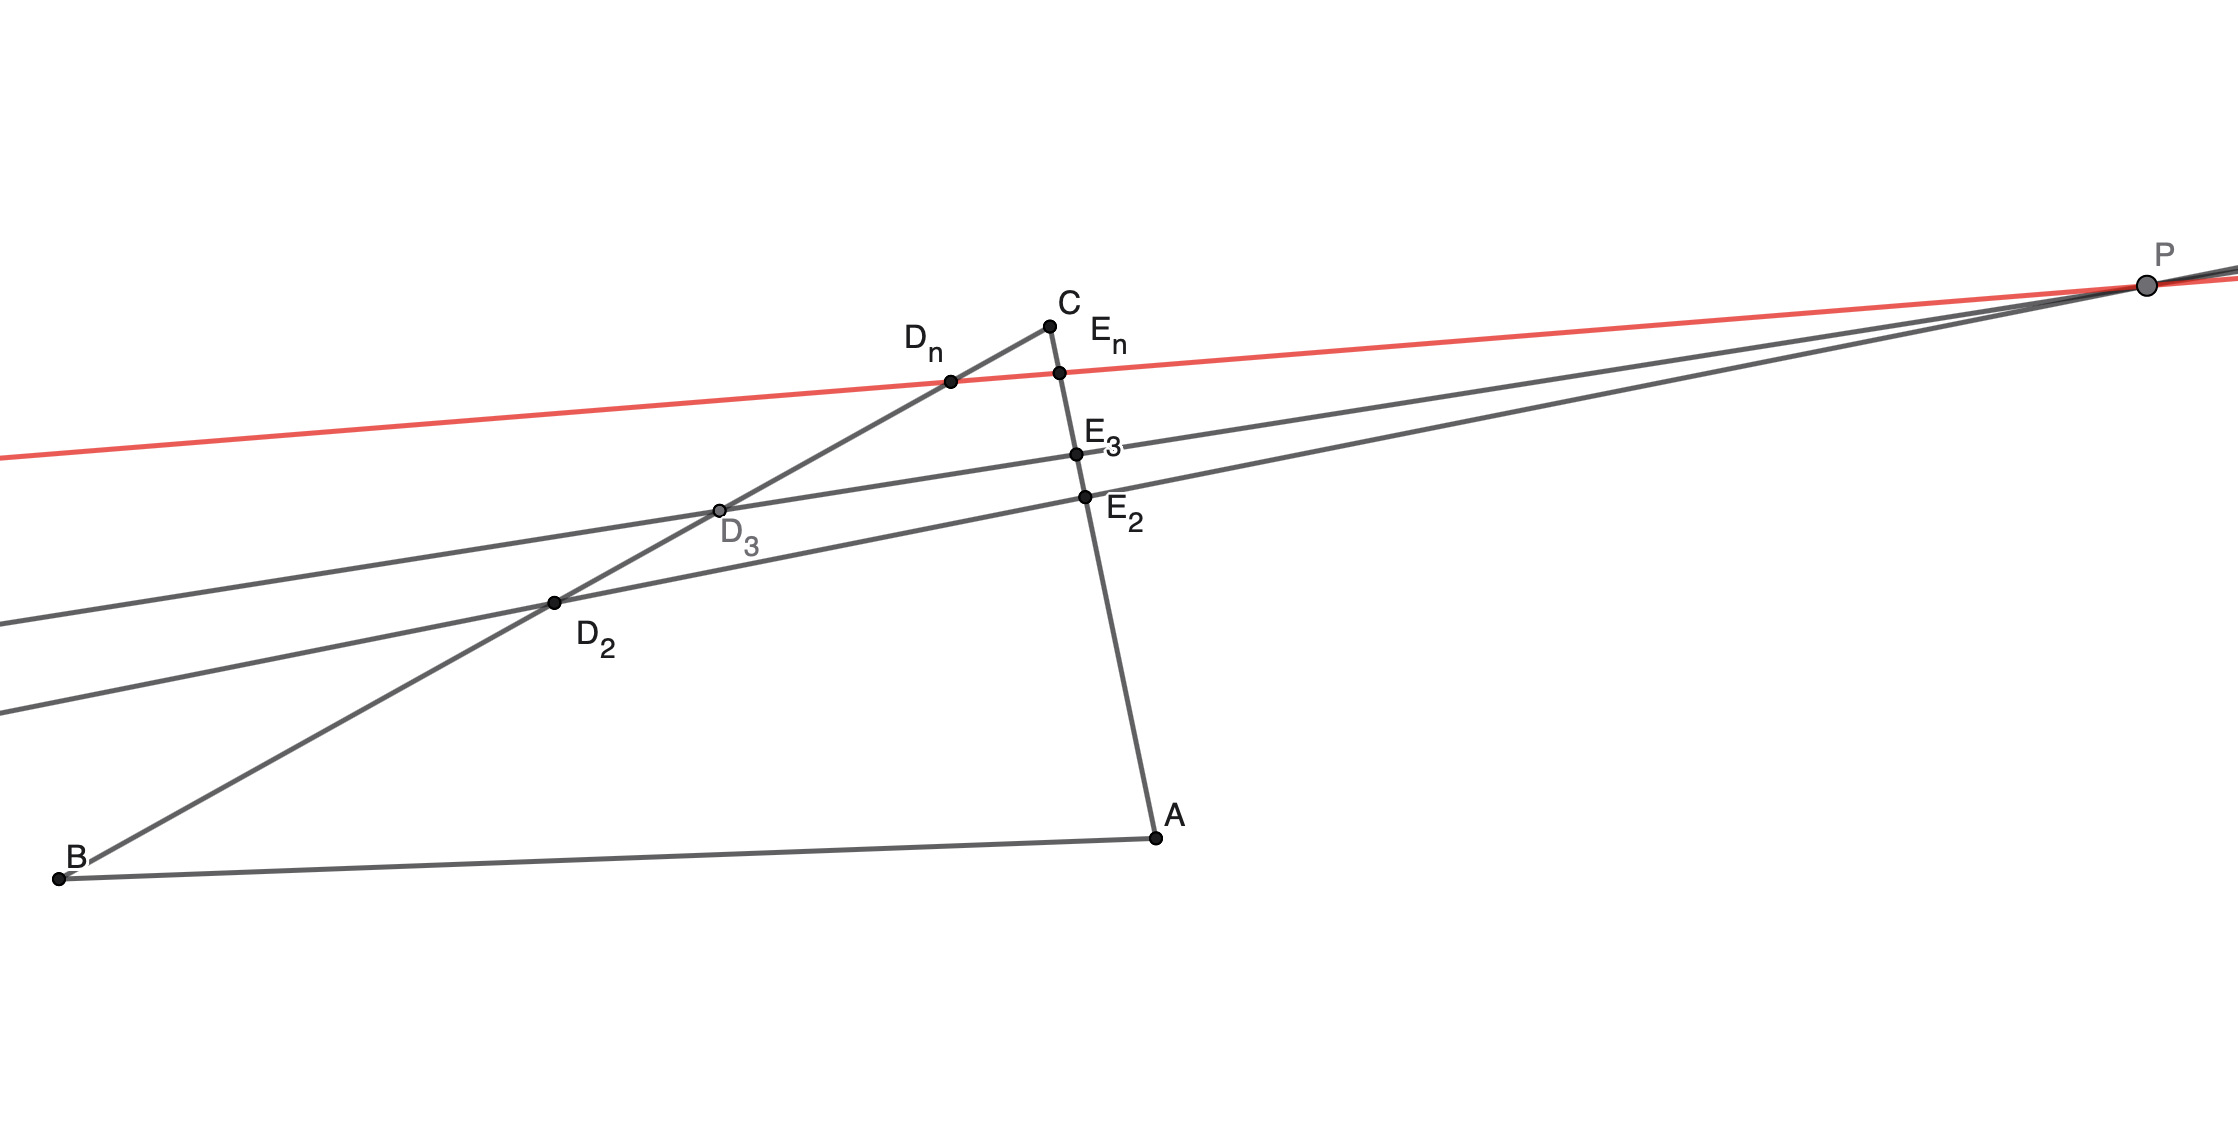
\includegraphics[width=1\linewidth]{ЭлМШ 2025-2026//VI блок//10/KMO_pic.png}
        \caption{\href{https://www.geogebra.org/calculator/sz9zg2hb}{Ссылка}}
        \label{fig:placeholder}
    \end{figure}

    \newpage

    \hspace{3mm}
    
    Посчитаем теперь двойные отношения четверок точек $(C, D_n, D_3, D_2)$ и $(C, E_n, E_3, E_2)$. 

    $$
    (C, D_n, D_3, D_2) = \frac{\overline{CD_3}}{\overline{D_3D_n}}: \frac{\overline{CD_2}}{\overline{D_2D_n}} = \frac{\frac{1}{3}CB}{\frac{1}{3}CB - \frac{1}{n}CB} : \frac{\frac{1}{2}CB}{\frac{1}{2}CB - \frac{1}{n}CB} = \frac{n}{n-3}:\frac{n}{n-2} = \frac{n-2}{n-3}
    $$

    $$
    (C, E_n, E_3, E_2) = \frac{\overline{CE_3}}{\overline{E_3E_n}}: \frac{\overline{CE_2}}{\overline{E_2E_n}} = \frac{\frac{1}{4}CA}{\frac{1}{4}CB - \frac{1}{n+1}CB} : \frac{\frac{1}{3}CB}{\frac{1}{3}CB - \frac{1}{n+1}CB} = \frac{n+1}{n-3}:\frac{n+1}{n-2} = \frac{n-2}{n-3} 
    $$

    Стало быть $(C, D_n, D_3, D_2)=(C, E_n, E_3, E_2)$, а значит по выше упомянутой лемме прямые $D_2E_2, D_3,E_3, D_nE_n$ пересекаются в одной точке.

    
\end{proof}